%discussion
\documentclass[../../main/main.tex]{subfiles}

\begin{document}
\title{Discussion}

%%%%%%%%%%%%%%%%%%%%% Chapter Discussion %%%%%%%%%%%%%%%
\chapter{Discussion}\label{chp:discussion}
The previous chapters describe the application of \gls{storm} to the patrol base operations.  This chapter elaborates on the \gls{stpa} and \gls{csbd} analyses by discussing findings not covered in previous chapters.   It then concludes with some discussion of challenges of the approach and how they are overcome.


      %%%%%%%%%%%%%%%%%%% Section STPA  %%%%%%%%%%%%%%%%%%
\section{STPA Analysis}\label{sec:stpadiscussion}

      %%%%%%%%%%%%%%%%%%% Section CSBD  %%%%%%%%%%%%%%%%%%
\section{CSBD Analysis}\label{sec:csbddiscussion}

\subsection{Authentication}
Authentication for this model of the patrol base operations is assumed through visual recognition of an authority.  But, in many parts of the patrol base operations, soldiers are challenged and must provide a password.  \gls{csbd} manages passwords (and cryptographic functions for automated systems) using a cryptographic secure state machine.  Such a parametrizable secure state machine already exits and it would be straight forward to apply it to future patrol base operations or to other non-automated, human-centered systems.

\subsection{Roles}
Principals in this model are roles (i.e., Platoon Leader, Platoon Sergeant, etc.).  But, a more accurate description would include soldiers acting in the role of a principal.  \gls{csbd} manages principals acting in roles using various \gls{acl} rules and a specific secure state machine.  Like cryptographic functions, such a parametrizable secure state machine already exists.  It would be straight forward to apply it to future patrol base operations or to other non-automated, human-centered systems.




      %%%%%%%%%%%%%%%%%%% Section Soldiers, etc. %%%%%%%%%%
 \section{Soldier, Squad, and Platoon Theories}
The model describes transitions among phases of the operations.  Additional models could include soldiers, squads, and platoon modules.  Figure \ref{soldierMission} is a possible description of a high level soldier module with one level expanded.  This is a simplified model to demonstrate the idea of a soldier module.  

\begin{figure}[h]
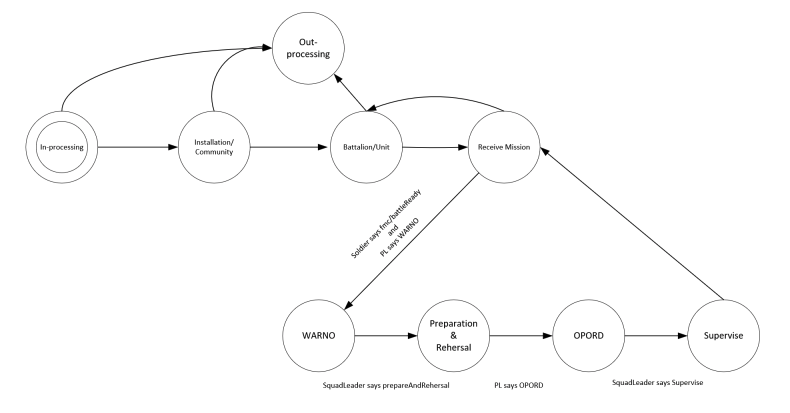
\includegraphics[width=\textwidth]{../figures/soldierMission}
\caption{\label{soldierMission}An abbreviated concept for a soldier module.}
\end{figure}

The soldier begins in the in-processing state.  She is then assigned to installation or community in-processing.  Then, she is assigned to a battalion or unit.  From there, she is sent on a mission or sent to out-processing.  From the mission state, she can be sent to out processing or proceed through the mission.  The mission begins in the planning phase where she receives her WARNO, prepares and rehearses, receives her OPORD, and is then supervised.  The ReceiveMission state would lead to other activities within the patrol base operations.

This is a basic idea of a soldier secure state machine.  It requires more research into the processing and soldier steps.  But, it is another way of thinking about the patrol base operations in terms of complete mediation.

The reader could imagine similar secure state machines for the platoon, squad, and team levels.  

 \section{Non-sequential Variations}
 The secure state machines described in the previous chapters describe mostly linear, sequential transitions.  But, non-linear and non-sequential secure state machines may describe some of the operations more accurately.  One example of non-linear, non-sequential operations is described in the planning secure state machine at the sub-level.  That secure state machine is shown again in figure \ref{ssmPlanPBDiagram2}.
 
 \begin{figure}[h!]
\centering
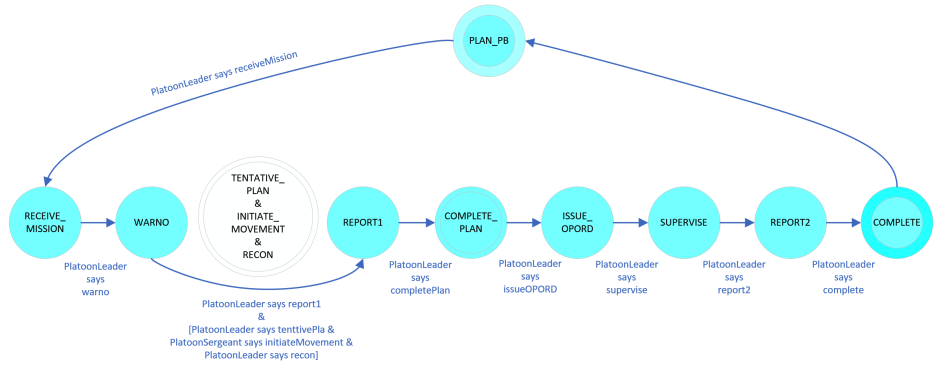
\includegraphics[width=\textwidth]{../figures/ssmPlanPBDiagram}
\caption{\label{ssmPlanPBDiagram2} Horizontal slice: PlanPB diagram.}
\end{figure}

For this state machine, three of the states could be completed in any order.  But, they ALL must be completed before completing the plan.  These states are TENTATIVE_PLAN, INITIATE_MOVEMENT, and RECON.   The secure state machine in figure \ref{ssmPlanPBDiagram2} describes these as "virtual states"  and simply requires their completion to be part of the input to the transition request.  


 \begin{figure}[h!]
\centering
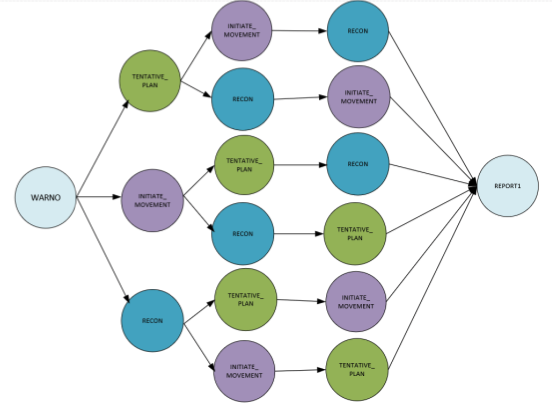
\includegraphics[width=\textwidth]{../figures/planAlt}
\caption{\label{planAlt} Alternative path through the three non-sequential states.}
\end{figure}

Another approach to modeling this section of the secure state machine is shown in figure \ref{planAlt}.  This diagrams show all permutations of paths from the WARNO state to the REPORT1 state. From the WARNO state, the operations can move to one of the TENTATIVE_PLAN, INITIATE_PLAN, or RECON states.  From there, the operations can move to any one of the two states that is has not yet occupied.  Finally, the operations move to the state it hasn't occupied yet.  There are a total of 6 paths from WARNO to REPORT1.

Another approach to modeling non-linear sequential states is to allow more transitions. For example, the top level progresses from the PLAN_PB state sequentially through to the COMPLETE_PB state.  But, it is possible that a platoon receives orders to move to the objective rally point before receiving a mission.  Figure \ref{toplevelAlt} shows an example of how to model this as a secure state machine. 

 \begin{figure}[h!]
\centering
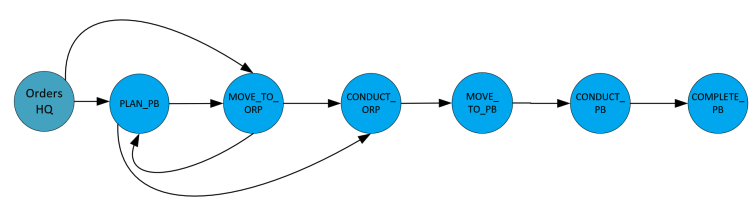
\includegraphics[width=\textwidth]{../figures/toplevelAlt}
\caption{\label{toplevelAlt} Permutation paths through the three non-sequential states..}
\end{figure} 
 
The additional arrows allow for the platoon to receive orders from head quarters and move directly to the objective rally point before the planning phase is complete. From there, the platoon can move into the planning phase and then conduct activities at the \gls{orp}. 

Additionally, the planning phase could begin while moving to the objective rally point.  This would eliminate encapsulation of each module, but it would be a more accurate description and the hierarchy could remain in-tact.  

\section{Concluding Comments}
\gls{storm} works.  Applying it to a non-automated, human-centered system is straight forward.  

The biggest challenge is managing the large size of the operations.  The patrol base operations are composed of numerous activities.  This challenge is dealt with using a modularized hierarchy of secure state machines.

The next biggest challenge for the \gls{stpa}/\gls{stpasec} analysis is expertise.  A subject matter expert\footnote{A subject matter expert was available for the modularized hierarchy of secure state machines.  But, he was not available for the \gls{stpa} analysis.  The author learned \gls{stpa} and patrol base operations simultaneously.} is necessary to describe the scenarios and causes of accidents and vulnerabilities.  For the \gls{csbd}, a subject matter expert is necessary to interpret the Ranger Handbook \cite{rangermanual} into secure state machines. 


Another challenge is managing complexity.  Some activities should be conducted in a sequential, checklist-like fashion.  But, others may be conducted in a variety of orders.  In addition, there is more than one type of patrol bases.  The Ranger Handbook describes the three types of patrol base as combat, security, and reconnaissance.  A complete model of the patrol base operations is beyond the scope of this master thesis.  But, it is doable and not much more involved than the model described in this master thesis.  

With the modularized hierarchy of secure state machines, large and complex systems non-automated, human-centered systems can be managed.  The model described in this master thesis is just a starting point and intended to demonstrate feasibility.  But, a full analysis of a system of this size and variety would start here and then adjust the transitions and details to accommodate.  

One of the biggest take homes from a design perspective is thinking critically about the system's security.  The detailed analysis of the system from the perspective of hazard and security analysis and complete mediation is informative.  

The next chapter discusses future work and some ideas about partial automation of the system with regards to accountability applications.
 

\end{document}